\chapter{T cell clonal diversity and pathogen immune escape}
\label{sec:VE}

The work presented in this chapter, apart from the preface, constitutes our manuscript in preparation titled ``\secbfcolor{T cell receptor repertoires with reduced N-nucleotide diversity may be more susceptible to pathogen immune escape}'' by H. Jamaleddine, J.N. Mandl, and A. Khadra. The title and contents of the manuscript that constitutes this chapter are subject to change, pending experiments in progress for testing the model predictions presented herein.


\phantomsection
\section*{Preface}
\addcontentsline{toc}{section}{Preface}

The work presented in Chapter~\ref{sec:AvC}, a result of collaborative efforts between modelling and experiments, has helped to uncover a novel benefit for TCR repertoire diversification by TdT, namely that lower-affinity T cells preferentially generated by TdT are better suited for the control of chronic pathogen replication. Importantly, however, neither experiments nor model ruled out the possibility that TdT may be serving other roles; thus, as a follow-up to this study, we sought to investigate a different hypothesis for the benefit of TCR repertoire diversification by TdT. Specifically, we asked whether TdT deficiency might result in ``holes'' in the TCR repertoire that mutating pathogens can more easily exploit, thus leaving the host more susceptible to T cell escape (discussed in Chapter~\ref{sec:intro_immuneEscape}). The work detailed in this chapter outlines what we have done to theoretically test this hypothesis, by adapting our model of T cell-mediated pathogen control to include stochastic mutation events with the goal of studying how varying the number of unique TCR clonotypes can affect within-host pathogen evolution.

\newpage
\section{Abstract}

T cell receptors (TCRs) expressed on the surface of T cells detect the presence of invading pathogens and allow them to mount efficient anti-microbial responses. Indeed, a sufficiently diverse TCR repertoire is necessary to respond to the wide range of pathogens that the host may encounter. These pathogens, on the other hand, may accrue mutations during infection in order to evade this response and persist within the host. While the tug-of-war between T cell-mediated control and pathogen evolution has far-reaching consequences on the progression of infectious diseases, little is known as to how TCR repertoire diversity affects the likelihood of “immune escape” by pathogens. In particular, it has been suggested that deficiency in terminal deoxynucleotidyl transferase (TdT), a DNA polymerase responsible for $\sim$90\% of TCR diversity, might lead to higher mutational burdens than in TdT-sufficient contexts, though this hypothesis has never been tested before. Here, we computationally investigated how TCR repertoire diversity impacts the balance between pathogen control versus immune escape by constructing a population model of pathogen evolution under T cell selective pressure. The model revealed that higher frequencies of dominant pathogen variants can, in some cases, emerge at intermediate levels of T cell diversity, and that these variants are less likely to be recognized by responding T cells. Our analysis further showed that pathogen intrinsic dynamics together with T cell control and selective pressure are all important determinants in the rate of immune escape. These results thus suggest a possibility for TdT-deficient T cell repertoires to be less effective against a mutating pathogen, providing theoretical support for the hypothesis that TCR diversification by TdT offers some protection from immune escape and could have implications, not only for individual hosts, but also at an epidemiological scale. 

\section{Introduction}

In recent years, the COVID-19 pandemic has motivated the emergence of a tremendous body of literature aimed at predicting pathogen evolution and spread using a host of mathematical and computational tools~\cite{saleem2022machine, rahimi2021review}. While many of these models study the epidemiology of transmission within and across populations, a complete understanding of pathogen evolution necessitates study at all scales, ranging from the molecular (e.g., mutation/recombination) and cellular (transmission of the pathogen from infected cells to susceptible cells and tissues) levels, all the way up to populations (transmission within and across communities) and global scales (e.g., migration patterns across large distances)~\cite{saad2022immuno}. Importantly, the immune system plays a key role in defining fitness landscapes for a pathogen evolving within a host~\cite{saad2022immuno,tenthorey2022evolutionary,moulana2023genotype}; therefore, studying how immune responses shape pathogen evolution is crucial to understanding infectious disease progression.

T cell-mediated immunity to infection in particular has been shown to impose Darwinian selection pressures on replicating viral pathogens, such as human immunodeficiency virus (HIV) and hepatitis C virus (HCV); this selection pressure in turn leads to the emergence of viral variants whose genomes have mutated in regions of their genomes presented to T cells in the context of peptide-major histocompatibility complex (pMHC)~\cite{walker2012t,petrovic2012hepatitis}, thus making them less recognizable to T cells that bind pMHC via their T cell receptors (TCRs). Despite the importance of studying the role T cells play in shaping pathogen evolution, the relationship between how many unique, pathogen-specific TCRs are present within the host (in other words, the host TCR repertoire diversity) and the rate of pathogen immune escape remains insufficiently described.

TCR repertoire diversity arises from somatic recombination of the antigen receptor gene during T cell development in the thymus by a complex sequence of events orchestrated by RAG1/2 protein complexes~\cite{schatz2011recombination}. In addition to the possible diversity conferred by combinatorial rearrangement of different V, D and J segments (for TCR \textbeta{}-chain) or V and J segments (for TCR \textalpha{}-chain), random nucleotide (N)-insertions between the junctions of these segments by terminal deoxynucleotidyl transferase (TdT) serves to further diversify the TCR repertoire $\sim$10-fold~\cite{schatz2011recombination,gilfillan1995mice,cabaniols2001most,litman2010origins,davis1988t,murugan2012statistical,zarnitsyna2013estimating}. Despite this impressive increase in TCR repertoire diversity as a result of TdT activity, the immunological advantage that this process confers has remained elusive. While our previous work showed that TdT-dependent T cells benefit the control of chronic replicating pathogens through the inclusion of TCRs with lower binding affinity for foreign pMHC~\cite{jamaleddine2022chronic}, we did not rule out whether diversification of the TCR repertoire via TdT may serve other purposes.

It has been previously proposed that TdT may be important for filling in ``holes'' in the TCR repertoire, thus making the host organism less susceptible to immune escape, for example in the context of a mutating pathogen~\cite{vrisekoop2014revisiting}. TCR sequencing in chimpanzees infected with HCV revealed that lower TCR\textalpha{} and TCR\textbeta{} chain diversity is associated with CTL escape and establishment of persistent infection as compared to a subject that resolved the infection~\cite{meyer2004limited}. This raises the question of whether reduced, but not absent, TCR diversity can causally promote greater mutational burden. Interestingly, there is some evidence to suggest that immune escape might occur maximally when the number of responding T cell clonotypes is lower. A theoretical study on cytotoxic T lymphocyte (CTL) responses to HIV suggested that, under certain conditions, the median number of escape events peaks when the number of epitopes recognized by CTLs is at an intermediate level~\cite{van2013rate}. Similarly, a simple model of pathogen adaptation to immune responses suggested that when immune pressure is intermediate, insufficient pathogen control/clearance, together with higher strength of selection for mutant variants, maximizes the likelihood of immune escape~\cite{grenfell2004unifying}.

In this work, we further explore this question by developing a computational model of the T cell response to a mutating pathogen, to theoretically test whether reduced, but not absent, TCR diversity can indeed promote higher rates of immune escape. We found that, under some parameter combinations, intermediate TCR diversity can indeed generate higher numbers of ``dominant" escape mutants that surpass a detection threshold. Consistent with previous work, we also showed that this effect is due to a combination of pathogen intrinsic propensities for generating mutant progeny, and that it is modulated by a balance between pathogen control/clearance and T cell selection pressure. Our results thus suggest a possibility for TdT-deficient T cell repertoires to be less effective at controlling pathogen mutation, providing theoretical support for the hypothesis that TCR diversification by TdT offers some protection from immune escape.

\section{Results}

\subsection{Computational model simulates pathogen evolution under selective pressure from TCR repertoire diversity}

To study the effect of TCR repertoire diversity on pathogen immune escape, we developed a computational model of pathogen replication and mutation coupled to a pool of reactive T cells with a varying number of unique TCR clonotypes, $N$ (Fig.~\ref{fig:VE_scheme}A, see Methods for detailed model description). T cell dynamics include constant input from the thymus, pathogen-induced proliferation, natural turnover, and intra- and inter-clonal competition for antigen and resources (with the former competition rate assumed to be greater than the latter).%
%
\begin{figure}[tb]
    \centering
    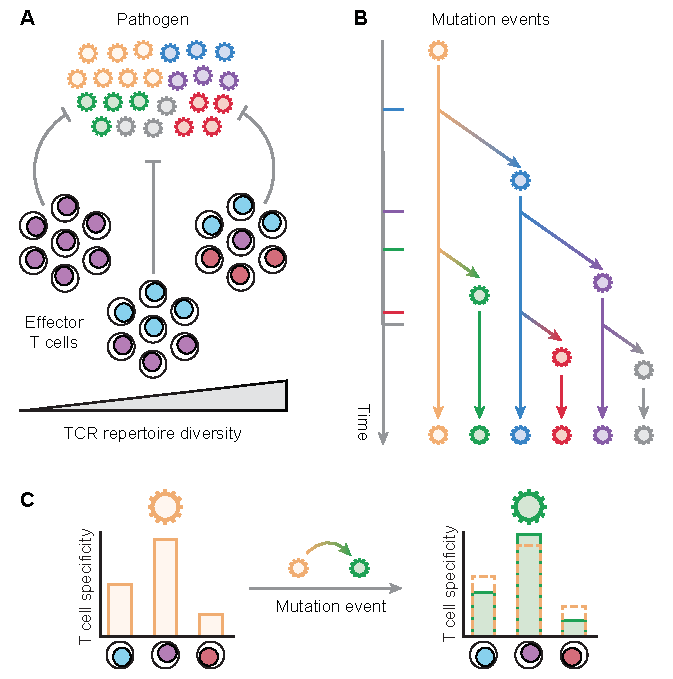
\includegraphics[width=0.64\textwidth]{Figures/VE/fig1_scheme.pdf}
    \caption[Computational population model of effector T cell diversity in response to a mutating pathogen]{\textit{Computational population model of effector T cell diversity in response to a mutating pathogen}. %
    %
    \secbfcolor{(A)}~Schematic illustrating effector T cells of varying TCR repertoire diversity responding to different variants of a replicating pathogen. %
    %
    \secbfcolor{(B)}~The pathogen is allowed to mutate within the model; the likelihood of a mutation event is proportional to the abundance of the parent strain. %
    %
    \secbfcolor{(C)}~Each T cell clone is assigned a value equivalent to the specificity of that clone for a pathogen strain. Upon mutation, the specificity of a T cell clone for a mutant strain is perturbed relative to its specificity for the parent strain.}
    \label{fig:VE_scheme}
\end{figure}
%
In the model, pathogen strains can give rise to mutant daughter strains throughout the infection (Fig.~\ref{fig:VE_scheme}B), with a mutation rate that is proportional to the abundance of the parental strain (i.e., strains with high pathogen loads are more likely to generate mutant progeny than ones with lower pathogen loads). To every pair of T cell clones and pathogen strains, we assign a value representing the specificity of that clone for that strain of the pathogen. Upon mutation, the specificity of any T cell clone for the daughter strain is assumed to be a small deviation in magnitude from its specificity for the parental strain (Fig.~\ref{fig:VE_scheme}C).

By simulating the model with one initial strain of the pathogen and $N=100$ unique TCR clonotypes, we generated time series showing different strains of the pathogen emerging in succession (Fig.~\ref{fig:VE_timeSeries}A) and the resulting T cell response across all clonotypes (Fig.~\ref{fig:VE_timeSeries}B). When quantifying the number of clonotypes whose cell numbers represent 95\% of the total responding T cell count, a metric that we used to measure the diversity of the responding T cell population at any given point in time, we found that clonotype diversity contracts at later time points relative to peak infection (Fig.~\ref{fig:VE_timeSeries}C); this is consistent with previous observations in early vs. late stages of infection with LCMV-Cl13~\cite{chang2020t}. Of note, the imbalanced, upward-branching architecture of the phylodynamic tree constructed from these simulations confirmed that the pathogen is indeed evolving under selective pressure exerted by T cells~\cite{volz2013viral}. Given that the model was able to reproduce TCR clonotype dynamics in the context of chronic infection and pathogen evolution under T cell pressure, we could thus begin to probe how mutational burden (i.e., the number and abundance of emerging pathogen variants) is affected by this selective pressure.
%
\begin{figure}[t]
    \centering
    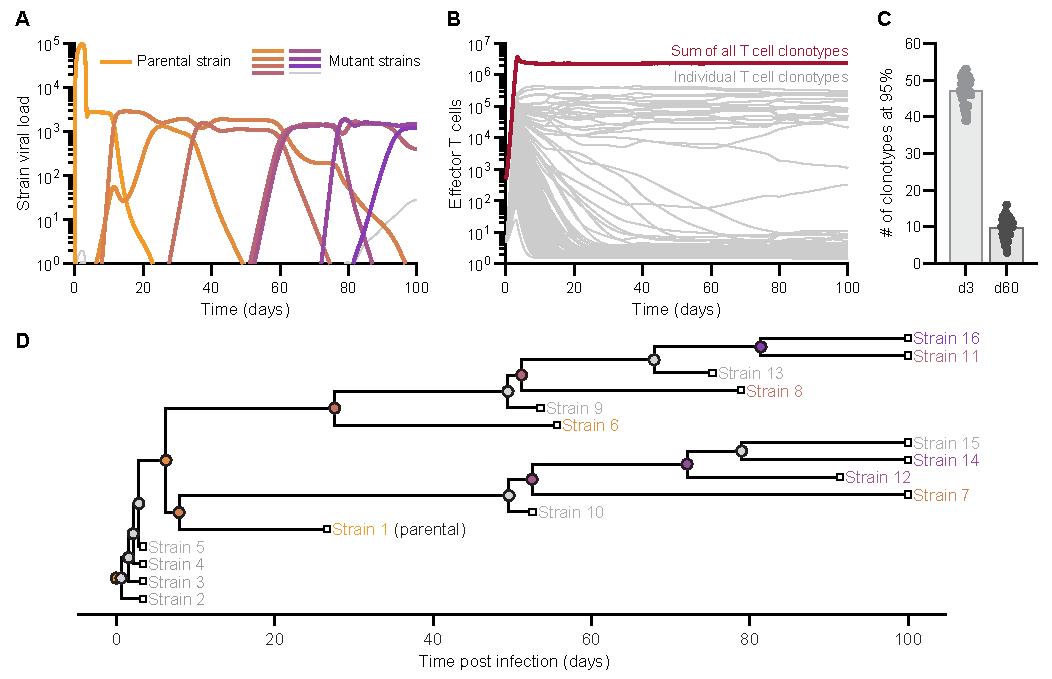
\includegraphics[width=\textwidth]{Figures/VE/fig2_timeSeries.pdf}
    \caption[Model simulations of the T cell response to mutating pathogen captures contraction of clonotype diversity over time]{\textit{Model simulations of the T cell response to mutating pathogen captures contraction of clonotype diversity over time}. %
    %
    \secbfcolor{(A)}~Pathogen load for each individual strain obtained from a single realization simulated by the model, starting from a single parental strain (Strain 1). Dominant strains (colored curves) are distinguished from those lowly abundant ones (gray curves) that make up $<$2\% of the pathogen pool at any given time. %
    %
    \secbfcolor{(B)}~Total number of effector T cells over time (red curve), comprised of 100 individual T cell clonotypes (gray curves) obtained from one single realization simulated by the model. %
    %
    \secbfcolor{(C)}~Number T cell clonotypes that make up 95\% of the responding T cell population at early vs. late stages of a chronic infection, computed from 50 independent realizations of model simulations. %
    %
    \secbfcolor{(D)}~Phylodynamic tree showing pathogen evolution over time. Strains are numbered according to their order of appearance and color-coded according to the traces shown in A. %
    }
    \label{fig:VE_timeSeries}
\end{figure}


\subsection{The number of dominant mutants is distinct from the total mutation rate}

Previous work has shown that the frequency of LCMV-Cl13 viral mutants 39 to 75 days post-infection in RAG2\KO{} mice (lacking both functional T and B cells) are negligible when compared to those in WT mice~\cite{smyth2021characterization}. Having developed our model of pathogen evolution, we asked whether the model produces similar results when simulated in the presence or absence of the effector T cell pool. To test this, we first simulated 200 independent realizations of the model in the absence of T cells or with $N=100$ unique T cell clonotypes, starting with a single parental strain, and quantified the cumulative number of strains of the pathogen that emerges over the course of each simulation (Fig.~\ref{fig:VE_noTcells}A,~B). Seemingly in contrast to the data from LCMV-Cl13 infections in RAG2\KO{} mice, we observed a greater absolute number of mutants over the course of an infection in the absence of T cells in the model (Fig.~\ref{fig:VE_noTcells}B). In fact, the number of total strains mirrored the simulated pathogen loads, with higher levels of pathogen obtained in the absence than in the presence of T cells  (Fig.~\ref{fig:VE_supp_noTcells}A). We experimentally verified this result by quantifying LCMV-Cl13 viral titres in WT and TCR\textbeta{}\KO{} mice 14 days post-infection, finding that indeed TCR\textbeta{}\KO{} mice possessed higher LCMV-Cl13 glycoprotein (GP) RNA levels relative to WT mice (Fig.~\ref{fig:VE_supp_noTcells}B,~C). This direct relationship between pathogen load and the total strain count in the model was not surprising, given that the rate of mutation was assumed to scale linearly with pathogen abundance in the model.
%
\begin{figure}[t]
    \centering
    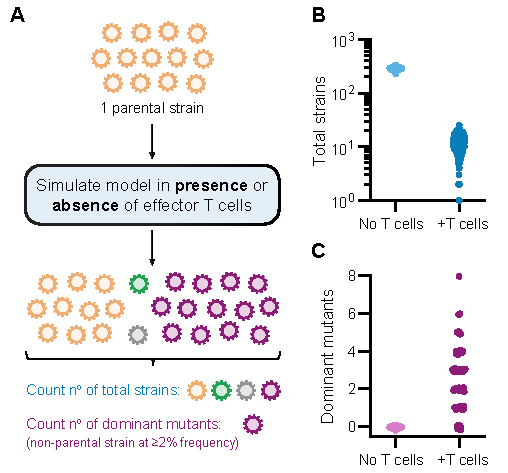
\includegraphics[width=0.48\textwidth]{Figures/VE/fig3_noTcells.pdf}
    \caption[Absence of selective pressure by T cells results in lack of dominant mutants despite high mutation rates]{\textit{Absence of selective pressure by T cells results in lack of dominant mutants despite high mutation rates}. %
    %
    \secbfcolor{(A)}~A schematic illustrating how model simulations are performed in the presence and absence of effector T cells, starting with a single parental strain. The total (i.e. cumulative) number of strains and the number of dominant mutants (non-parental strains present at a frequency of at least 2\% at any point of the simulation) appearing throughout the simulation are quantified. %
    %
    \secbfcolor{(B,C)}~Total number of strains (B) and number of dominant mutants (C) arising by 100 days post-infection predicted by the model, in the absence of T cells or when the number of T cell clones $N$ is set to 100. Data shown result from 200 independent realizations of model simulations.%
    }
    \label{fig:VE_noTcells}
\end{figure}
%

In light of the apparent discrepancy regarding mutational burden between our model and data from RAG2\KO{} mice, we reasoned that a more biologically relevant metric would not be the total number of mutants, but rather those that are sufficiently abundant (or ``dominant") relative to the overall pathogen load since these mutants would presumably have a greater impact on the infected host and on disease transmission at the epidemiological scale. Furthermore, it is worth noting that variants present at low relative abundances cannot be reliably detected using conventional sequencing techniques. Indeed, it has been estimated that variants present at a frequency below $\sim$2\% cannot be confidently identified~\cite{lauring2020within}, although this threshold value for variant identification is not fixed but rather strongly dependent on the input genome size~\cite{mccrone2016measurements}, among other factors. Based on this argument, we decided to instead quantify the number of ``dominant'' mutants, defined as the variants of the parental strain that each constitute a minimum of 2\% of the total pathogen load at any given time throughout the simulation. Indeed, when we quantified the number of dominant mutants predicted by the model with or without effector T cell control, we found no dominant mutants arise in the absence of T cells, despite a larger number of total strains (Fig.~\ref{fig:VE_noTcells}A,~C). This finding thus agrees with previous data showing a lack of measured mutational burden in the absence of selective pressure from adaptive immunity~\cite{smyth2021characterization}, and highlights the importance of distinguishing dominant mutants from other, more lowly abundant variants in subsequent model analyses.

\subsection{Intermediate TCR repertoire diversity can lead to higher numbers of dominant mutants that evade the T cell response \textit{in silico}}

\begin{figure}[b!]
    \centering
    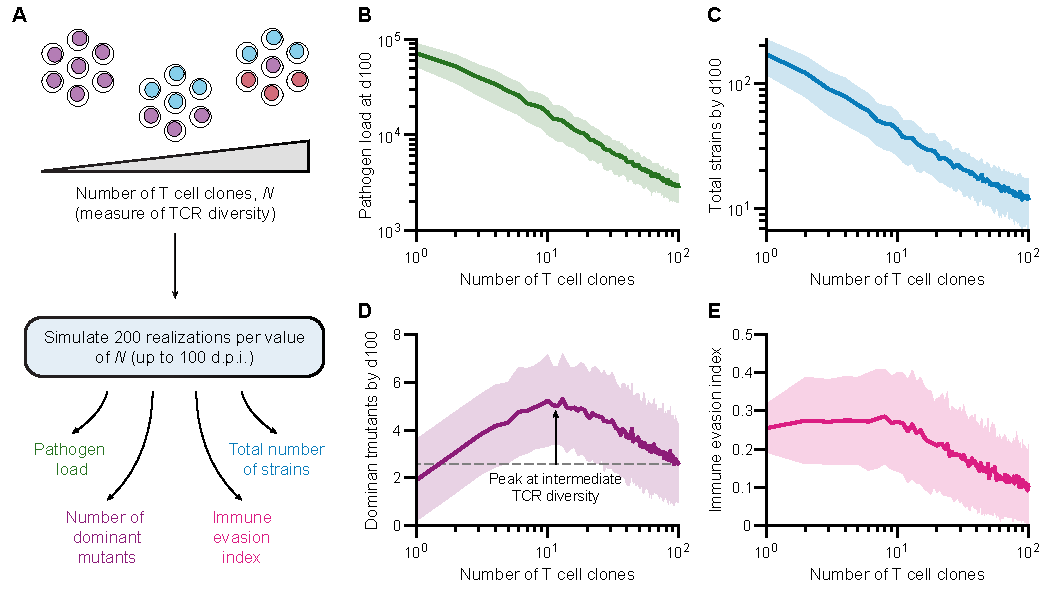
\includegraphics[width=\textwidth]{Figures/VE/fig4_effectOfN.pdf}
    \caption[Intermediate level of TCR repertoire diversity in the model promotes greater levels of immune escape]{\textit{Intermediate level of TCR repertoire diversity in the model promotes greater levels of immune escape}. %
    %
    \secbfcolor{(A)}~A schematic illustrating how model simulations are performed when the number of effector T cell clones, a parameter representing TCR diversity in the model, is gradually varied to test its effect on pathogen replication and evolution over time. %
    %
    \secbfcolor{(B,~C)}~Simulations of pathogen load by day 100 post-infection~(B) and total number of pathogen strains that emerges over the course 100 days~(C) as a function of the number of T cell clones considered in the model. %
    %
    \secbfcolor{(D,~E)}~Number of dominant mutants (D), defined as the number of strains other than the starting strain with $\geq$2\% abundance at any point in time, and pathogen evasion index (E), representing the degree with which escape mutants evade T cell recognition, as a function of the number of T cell clones. Dashed line in D indicates the average number of dominant mutants for $N=100$. Curves in panels B-E represent the mean over 200 realizations of model simulations, and shaded areas represent $\pm$ standard deviation. %
    }
    \label{fig:VE_effectOfN}
\end{figure}
Having verified model outcomes at the two ends of the T cell diversity spectrum (i.e., when there are no T cells or there are many unique T cell clones), we next asked how gradually varying the number of T cell clonotypes impacts pathogen evolution across this spectrum  (Fig.~\ref{fig:VE_effectOfN}A). In doing so, we found that the total pathogen load and, consequently, the total number of strains that emerge over the course of the simulated 100-day period were inversely proportional to the number of T cell clones in the model (Fig.~\ref{fig:VE_effectOfN}B,~C), suggesting that more diverse TCR repertoires provide increased control of pathogen replication overall. Interestingly, however, when we quantified the number of dominant mutants as a function of TCR diversity, we found that more mutants emerge on average at intermediate levels of TCR diversity (Fig.~\ref{fig:VE_effectOfN}C).

Since we were interested in pathogen immune escape as a function of TCR diversity, we wondered whether responding T cells in the model were less specific overall for the mutants that do become dominant relative to the parental strain at intermediate TCR diversity values. To investigate this, we developed a metric that we termed the ``immune evasion index'', which measures the degree with which dominant mutants evade recognition by T cells in the model (see Methods). When calculating the value of this index as a function of TCR diversity, we indeed found that intermediate values of repertoire diversity not only promotes the formation of more dominant mutants (Fig.~\ref{fig:VE_effectOfN}D), but that these mutants are less recognizable by responding T cells than dominant mutants emerging at higher TCR diversity (Fig.~\ref{fig:VE_effectOfN}E). Importantly, however, this observation is dependent on model parameters; for example, gradually increasing \textit{inter}-clonal competition to be identical to \textit{intra}-clonal competition among responding T cells abolishes this effect and the number of dominant mutants instead approaches a plateau as TCR diversity is increased (Fig.~\ref{fig:VE_supp_asymComp}). Nonetheless, these data suggest that insufficient TCR repertoire diversification might lead to more immune escape in certain parameter regimes, and that this observation has potential implications in the case of T cells lacking TdT-dependent N-nucleotide diversification.


\subsection{Optimal range of pathogen loads promote highest levels of mutational burden}

\begin{figure}[b!]
    \centering
    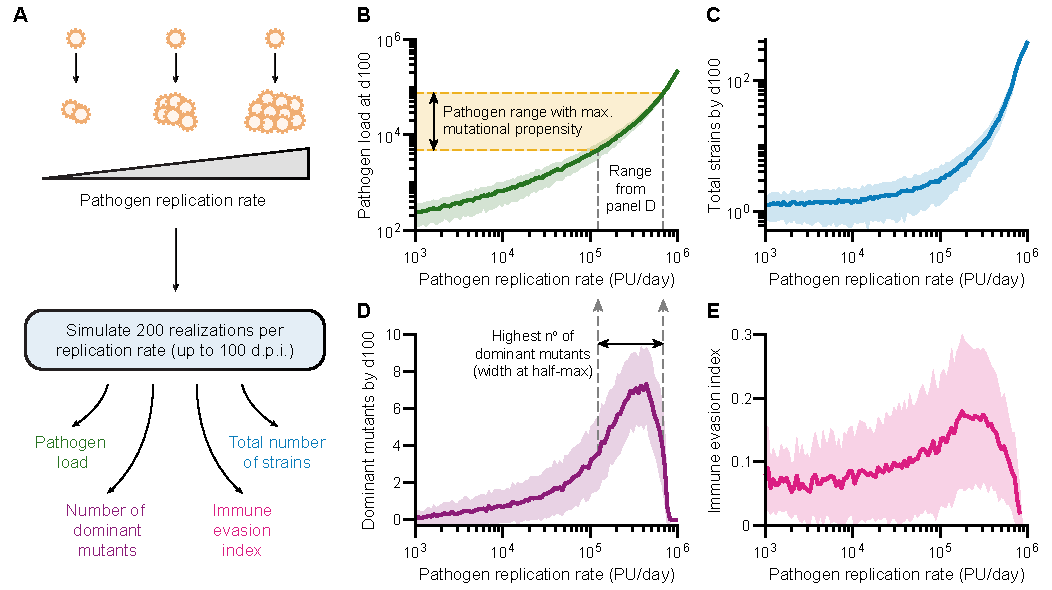
\includegraphics[width=\textwidth]{Figures/VE/fig5_effectOfBeta.pdf}
    \caption[High mutational burden and more immune escape occur within an optimal range of pathogen loads]{\textit{High mutational burden and more immune escape occur within an optimal range of pathogen loads}. %
    %
    \secbfcolor{(A)}~A schematic illustrating how model simulations are performed to investigate the effect of equilibrium pathogen loads on its evolution; the pathogen replication rate (parameter $r_P$ in the model, see Methods) is gradually increased and model outcomes are assessed as in Fig.~\ref{fig:VE_effectOfN}. The number of T cell clones, $N$, is held constant at a value of 50 clones. %
    %
    \secbfcolor{(B,~C)}~Simulations of pathogen load by day 100 post-infection~(B) and total number of pathogen strains that emerges over the course 100 days~(C) as a function of the rate of pathogen replication.
    %
    \secbfcolor{(D,~E)}~Number of dominant mutants (D), and pathogen evasion index (E), as a function of pathogen replication rate. The half-maximum width of the curve in D is used to determine the range of pathogen loads in B that maximally promote the emergence of dominant mutants (yellow-shaded region). Curves represent the mean over 200 realizations of model simulations, and shaded areas represent $\pm$ standard deviation.}
    \label{fig:VE_effectOfBeta}
\end{figure}

In light of our observations thus far, we wished to further investigate the reason for the divergent relationship between \textit{dominant} mutant emergence as compared to pathogen load and the \textit{total} number of mutants. Based on previous modelling work~\cite{grenfell2004unifying}, we hypothesized that there exists an optimal zone of pathogen load where the amount of replicating pathogen is high enough to maintain a high mutation rate, but also low enough that new, more evasive mutants can readily overtake the strains that are dominant upon its emergence. To directly test this, we checked whether we would observe similar results by gradually increasing equilibrium pathogen loads in the model, while keeping all other parameters constant. Since we do not have an explicit parameter representing pathogen load, this was achieved by varying the pathogen replication rate parameter ($r_P$, see Methods) (Fig.~\ref{fig:VE_effectOfBeta}A). Our results showed that, whereas pathogen loads and the total number of strains increase monotonically with increasing pathogen replication rates (Fig.~\ref{fig:VE_effectOfBeta}B,~C), the number of dominant mutants peaks before falling off sharply when both pathogen replication and loads are high (Fig.~\ref{fig:VE_effectOfBeta}D,~B). We observed a similar trend when we additionally quantified the immune evasion index (Fig.~\ref{fig:VE_effectOfBeta}E), which mirrors the number of dominant mutants by peaking at intermediate pathogen replication rates.

While the above model outcomes were measured as a function of pathogen replication rate, in this analysis, we used this parameter specifically to modulate pathogen load (Fig.~\ref{fig:VE_effectOfBeta}B). In order to relate these observations made with respect to pathogen replication rates back to pathogen loads, we determined what equivalent range of the latter promotes the highest levels of dominant mutants; to do this, we computed the width at half-maximum of the curve in Fig.~\ref{fig:VE_effectOfBeta}D, and determined the corresponding range of pathogen loads by relating it back to the curve in Fig.~\ref{fig:VE_effectOfBeta}B. We define this range of pathogen loads, resulting in more than half of the average maximum number of dominant mutants, as having maximal ``mutational propensity'' (Fig.~\ref{fig:VE_effectOfBeta}B). This range exists due to competition for replication between different strains of the model, which is a feature of the model that ensures accurate behaviour when multiple strains are present (see Section~\ref{sec:VE_modelDesign} -- Model design); briefly, when pathogen loads are high, competition for replication within target cells makes it less likely for newly emerged, lowly abundant mutants to overtake the existing pool of strains despite high mutation rates. In summary, the model suggests that an intermediate range of pathogen loads exists that maximally promotes the emergence of escape mutants, and that this results from a balance between sufficient rates of mutation and competitive dynamics among strains.

\subsection{The rate of immune escape depends on a balance between pathogen intrinsic and T cell-dependent mechanisms}

Our previous result suggests that changes in pathogen dynamics can alter the number of dominant mutants that emerge, with an optimal range of pathogen loads displaying maximal mutational propensity. However, we wondered whether we could tease apart the contributions to immune escape of the intrinsic properties of the pathogen vs. those that depend on T cell control, and how these processes interact to generate the model outcomes observed thus far. To investigate this, we gradually varied the number of T cell clones, and for each individual diversity value, we repeated the analysis described in the previous section to measure how maximal mutational propensity changes as a function of TCR diversity (Fig.~\ref{fig:VE_supp_maxMutProp}A). Interestingly, we found that more dominant mutants can emerge at higher numbers of T cell clones within the range of maximal mutational propensity (Fig.~\ref{fig:VE_supp_maxMutProp}B), indicating greater selection pressure exerted by T cells on pathogen evolution with increasing TCR diversity.

\begin{figure}[t!]
    \centering
    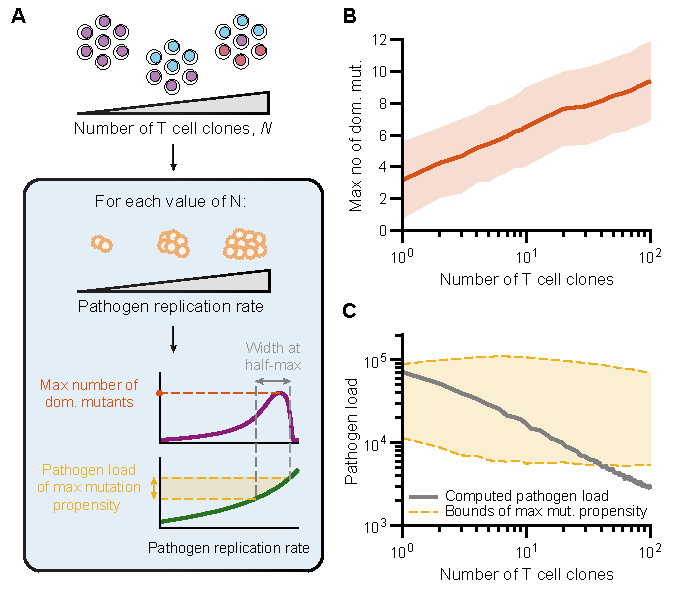
\includegraphics[width=0.64\textwidth]{Figures/VE/fig6_maxMutProp.pdf}
    \caption[Peak in number of dominant mutants at intermediate TCR diversities can be explained by the balance between pathogen control and T cell selective pressure]{\textit{Peak in number of dominant mutants at intermediate TCR diversities can be explained by the balance between pathogen control and T cell selective pressure}. %
    %
    \secbfcolor{(A)}~A schematic illustrating how model simulations are performed by gradually varying the number of T cell clones, $N$, and at each value of $N$ the relationship between pathogen replication rate and the number of dominant mutants is computed as described previously (Fig.~\ref{fig:VE_effectOfBeta}); the goal is to determine the maximum number of dominant mutants, and the range of pathogen loads with the highest mutational propensity, as a function of $N$. %
    %
    \secbfcolor{(B)}~The maximum expected number of dominant mutants is higher for higher TCR diversity, indicating that T cell control exerts more selective pressure on pathogens. Curve: mean, shaded region: standard deviation. %
    %
    \secbfcolor{(C)}~Despite higher selective pressure for large numbers of T cell clones, greater pathogen control decreases computed pathogen abundances (gray curve, identical to Fig.~\ref{fig:VE_effectOfN}B) below the range of pathogen loads with the highest mutational propensity (shaded region bounded by dashed lines).} 
    \label{fig:VE_supp_maxMutProp}
\end{figure}

However, while greater TCR diversity leads to more selection pressure on the evolving pathogen, we previously showed that increasing the number of T cell clones also reduces the total pathogen load (Fig.~\ref{fig:VE_effectOfN}B), and that the number of dominant mutants peaks at intermediate TCR diversities before coming back down when the number of unique clones is higher (Fig.~\ref{fig:VE_effectOfN}D). Thus, we wondered whether we could reconcile these findings by comparing the total pathogen load predicted by the model against the range of pathogen loads with maximal mutational propensity, both as a function of TCR diversity. Indeed, by overlaying the observed pathogen load (computed as shown previously in Fig.~\ref{fig:VE_effectOfN}B) onto the computed range within which higher numbers of dominant mutants arise (Fig.~\ref{fig:VE_supp_maxMutProp}C), we found that increasing the number of T cell clones drives pathogen loads below this range, thus explaining why fewer dominant mutants are observed than would be expected based purely on selection pressure alone. Of note, we observed that the range of pathogen loads with maximal mutational propensity is relatively independent of TCR diversity, suggesting that this range is intrinsic to pathogen replication dynamics. Taken together, these data suggest that while the optimal range of pathogen loads favouring the emergence of evasive dominant mutants is largely dependent on the intrinsic properties of the pathogen, different levels of T cell control can alter pathogen loads, and thus mutational burden, relative to this range. Hence, the peak in the rate of immune escape at intermediate TCR diversities can be explained by a balance between higher selective pressure on pathogen strains and insufficient control of pathogen replication.


\section{Discussion}

Despite the important role that T cell activity plays in shaping pathogen evolutionary landscapes, there has been surprisingly limited work aimed specifically at addressing how TCR diversity interacts with pathogen intrinsic dynamics to promote immune escape. Our modelling results propose that when the amount of pathogen falls within a specific range, its propensity for generating mutants that can then efficiently replicate within the host is maximized. We found that, while this range is largely independent of T cell control, it dictates how T cell diversity can influence pathogen evolution by modulating pathogen loads relative to this range. More specifically, our results revealed that while more T cell control can lead to higher evolutionary selection pressure on the mutating pathogen (driving the potential number of escape variants up), but it also lowers total pathogen loads, bringing the latter outside the intrinsic range of maximal mutational propensity and causing the number of escape variants to go down. In other words, the resulting mutational burden of the pathogen on the host will depend on the balance between these two opposing forces. We showed that a potential consequence of these interacting dynamics is a peak in the rate of immune escape at intermediate values of TCR diversity, with otherwise fewer dominant mutants being observed on average when the number of responding T cell clonotypes is comparatively lower or higher.

Importantly, our findings could have implications with regard to TCR repertoire diversification via TdT. While TdT-deficient hosts, with about 10-fold fewer unique T cell clonotypes~\cite{davis1988t,murugan2012statistical,zarnitsyna2013estimating}, were hypothesized to be more prone to immune escape by pathogens relative to their WT counterparts owing to the presence of repertoire ``holes''~\cite{vrisekoop2014revisiting}, no subsequent work has directly tested this hypothesis. Our model suggests that it is certainly plausible for higher rates of immune escape (in the form of dominant mutants) %with higher immune evasion indices in the model
to result from a 10-fold reduction in TCR repertoire diversity relative to baseline (Fig.~\ref{fig:VE_effectOfN}), provided that an increase in TCR diversity is accompanied by greater control of pathogen replication (and hence lower pathogen loads). We also know from our previous work that mice chronically infected with LCMV-Cl13 have higher viral loads than WT mice when TdT is lacking in their T cells~\cite{jamaleddine2022chronic}. One can thus infer, based on our model predictions, that LCMV-Cl13 viral loads might fall within the range of maximal mutational propensity that favours the production of escape variants in the absence of TdT. Using existing sequencing tools that can assess within-host pathogen diversity~\cite{lauring2020within}, subsequent experimentation will be able to test our model prediction to determine whether another evolutionary advantage of TdT is indeed to protect hosts from mutating pathogens.

Interestingly, it is known that T cells lacking N-nucleotide diversity from TdT are more cross-reactive than those with N-diversity, which was proposed as an explanation for the lack of TdT expression in neonates~\cite{gavin1995increased}. It should be noted that our model does not consider differences in cross-reactivity for less diverse TCR-repertoire or how this could impact the emergence of escape variants, though presumably incorporating such a mechanism might partially compensate for the lower number of unique clones and diminish the peak in the number of dominant mutants at intermediate diversity. We also showed that this effect was dependent on certain parameters of the model (including the ratio between inter- and intra-clonal competition), and that there exist regimes in parameter space where intermediate TCR diversities do not generate higher numbers of unique clones (Fig.~\ref{fig:VE_supp_asymComp}). It is thus important to note that the model does not definitively conclude that TdT-deficient TCR repertoires are more susceptible to immune escape by mutating pathogens, but rather suggests that these dynamics are theoretically possible and that this merits further investigation to confirm whether or not TdT benefits host immune responses by limiting escape.

While our model was kept simple in order to focus on the effects of T cell clonal diversity on pathogen immune escape, other elements that were not included explicitly also exert their effects on the evolutionary dynamics of pathogens that are worth noting. For example, our model assumes that pathogen replication rate is unchanged upon mutation, and that there is an equal chance for T cell specificity for the mutant strain to be higher or lower than that of the parent strain. However, it has been established in the context of viral quasispecies evolution that a large number of mutations are deleterious or even lethal for pathogens, and that overall fitness tends to decrease across generations~\cite{bergstrom1999transmission,peck2018complexities,wylie2011biophysical}. Thus, while incorporating the effect of more realistic fitness landscapes would increase the complexity of the model, it certainly remains of relevance to ask how such inclusions could affect predicted outcomes and how TCR diversity profiles impact pathogen evolution across realistic fitness valleys.

Our finding that the range of pathogen loads with maximal mutational propensity is largely invariant to different levels of T cell selective pressure was quite intriguing to us. Incidentally, earlier theoretical work on viral-immune co-evolution analogously showed that an optimal mutation rate exists that maximizes immune escape, and that the experimentally calculated per-genome average mutation rate of HIV-1 lies near this optimum~\cite{kamp2002viral}. It is thus conceivable that this notion extend to pathogen loads as suggested by our model, since the abundance of replicating pathogen will itself dictate the total number of mutations for a given mutation rate. Strikingly, however, while the mutation rate per base pair varies by orders of magnitude across different types of DNA and RNA viruses, when accounting for the entire genome size, the per-genome average mutation rate is relatively similar across different species of viruses~\cite{sanjuan2016mechanisms,peck2018complexities}. In spite of this, within-host viral phylogenies still vary substantially~\cite{grenfell2004unifying}. While this undoubtedly depends on many interconnected aspects of the pathogen biology and the resulting immune response, perhaps viral set points in HIV and HCV, which produce chronic infections in hosts and show substantial evidence of evolution in response to immune pressure~\cite{grenfell2004unifying, raghwani2019high,lemey2006hiv}, fall within these ranges of maximum mutational propensity so as to optimally adapt to the host immune landscape. 

In summary, by applying the principles of pathogen-immune co-evolution to specifically study the impact of TCR diversity on immune escape, interesting predictions arose from model results that are worth further experimental investigation. In addition, our observations led to intriguing insights that may extend beyond the scope of TCR diversity, having potentially broader implications to pathogen evolution more generally.

\section{Methods}

\subsection{Mice}

C57BL/6  and TCR\textbeta{}\KO{} mice~\cite{mombaerts1992mutations} were purchased from Jackson Laboratories (Bar Harbor, ME). % \red{The TdT\KO{} mice were shared by Dr. A. Feeney (The Scripps Research Institute)~\cite{gilfillan1993mice}}.
All mice were on a C57BL/6 background, bred in-house and experiments performed at 8-13 weeks of age with only males. Animal housing, care, and research were in accordance with the Guide for the Care and Use of Laboratory Animals and all procedures performed were approved by the McGill University Animal Care Committee.

\subsection{LCMV-Cl13 stock and infections}

The Clone 13 strain of LCMV was propagated from stocks provided by Dr. M. Richer (University of Indiana) on L929 cells, as described previously~\cite{jamaleddine2022chronic}. Mice were infected by injecting 2\E{6} plaque forming units (PFU) of LCMV-Cl13 intravenously as per established protocol~\cite{wherry2003viral,richer2013pathogen}. Mice were sacrificed 14 days post-infection, and their spleens were collected in 1\%~RPMI before being weighed and homogenized in Lysing Matrix D tubes (MP Biomedicals) using a MagNA Lyser (Roche) at 6000~rpm for 40~seconds. Spleen homogenate was then spun down at 12,000~rpm for 10 minutes at 4\degree{C}. To further clarify the solution, the supernatant was transferred to a new sterile tube and re-spun at 12,000 rpm for 10 minutes at 4\degree{C}, and 400~\textmu{}L of TRIzol reagent (Invitrogen) was added to 200~\textmu{}L aliquots of the supernatant from homogenized spleens before being stored at $-80$\degree{C} for RNA processing and quantification of viral titres.

\subsection{RNA extraction and viral titre determination}

To quantify viral loads in the spleens of WT or TCR\textbeta{}\KO{} mice, samples were thawed on ice before adding 80~\textmu{}L of chloroform, incubating at room temperature for 5 minutes, and spinning down at 12,000~rpm for 15 minutes. RNA was extracted using the PureLink RNA Mini Kit (Invitrogen), followed by cDNA conversion of 220~ng of RNA in 20~\textmu{}L reaction volumes with the High-Capacity cDNA Reverse Transcription Kit (Invitrogen). Viral titres were determined via qPCR to quantify LCMV-GP RNA levels using primers described previously~\cite{welsh2008lymphocytic}.

\subsection{Statistical analyses of experimental data}

Group comparisons were performed using MATLAB version 2022a. Information about implemented statistical tests and sample sizes for individual experiments is provided in the figure legends.

\subsection{Computational model}

\subsubsection*{Model formalism}
To model the dynamics of pathogen evolution as a function of TCR repertoire diversity, we constructed an ordinary differential equation (ODE) model consisting of $N$ fixed clones of effector T cells $E_i(t)$ ($i \in \{1,\,2,\,...,\,N\}$) and $M(t)$ strains of a mutating pathogen $P_j(t)$ ($j \in \{1,\,2,\,...,\,M(t)\}$), where the total number of pathogen strains, $M(t)$, is allowed to increase with time via random mutation events. The system of equations describing the model can be written as
%
\begin{align}
    \dv{E_i}{t} &= \frac{\sigma_E}{N} + r_E E_i \sum_{j=1}^{M(t)}\left(\frac{P_j}{P_\textup{tot} + k_{ij}} \right) -\delta_E E_i - \varepsilon E_i \sum_{n=1}^N \omega_{in} E_n, \label{eq:VE_E} \\[0.5em]
    \dv{P_j}{t} &= r_P \frac{P_j}{P_{\textup{tot}}+P_h} - \delta_P P_j - \kappa_P \sum_{i=1}^{N}\left(E_i \frac{P_j}{P_{\textup{tot}} + k_{ij}} \right). \label{eq:VE_P}
\end{align}

Equation~\eqref{eq:VE_E}, describing the rate of change of effector T cell clone $i$ over time, was adapted from previous models of T cell dynamics~\cite{jamaleddine2020quantifying,jamaleddine2022chronic,khadra2011investigating,jaberi2015continuum}. The source term $\sigma_E$ represents total thymic input of all pathogen-specific T cells; although different clonotypes are present at different precursor frequencies in the na\"{i}ve T cell repertoire~\cite{quigley2010convergent}, for simplicity we let thymic input be equally divided among all $N$ T cell clones. All clones are assumed to share a natural turnover rate given by $\delta_E$, and to proliferate with a maximum rate $r_E$ upon pathogen recognition. The contribution of each strain of pathogen, $P_j$, will depend on the abundance of that strain relative to the total pathogen load, denoted by $P_{\textrm{tot}} = \sum_j P_j$, and on the specificity of T cell clone $i$ for strain $j$, a value that depends reciprocally on the magnitude of the parameter $k_{ij}$. This latter parameter is sampled randomly from a log-normal distribution, with base-10 logarithmic mean $\mu_k$ and standard deviation $\sigma_k$. The final term in Eq.~\eqref{eq:VE_E} represents the rate of intra- and inter-clonal competition among T cells. We let the rate of intra-clonal competition be equal to $\varepsilon$, which represents competition for cognate antigen as well as other survival signals~\cite{khadra2009role,jamaleddine2020quantifying,jamaleddine2022chronic}, and let inter-clonal competition occur at a lower rate $f \times \varepsilon$, where $f<1$ (since different T cell clones may have different antigen specificity). In other words, we assumed that
%
\begin{equation*}
    \omega_{in} = 
    \begin{cases}
        1 \qquad \textrm{if} \qquad i=n, \\
        f \qquad \textrm{otherwise}.
    \end{cases}
\end{equation*}

The rate of change of each pathogen strain $P_j$ as a function of time is described by Eq.~\eqref{eq:VE_P}. We assumed that the \textit{per capita} replication rate of each strain is upper-bounded by the fraction $r_P/P_h$, and that, when pathogen loads are sufficiently high (i.e., when $P_{\textrm{tot}} > P_h$), more abundant strains have a higher probability of invading target cells and thus replicate more efficiently. We let $\delta_P$ be the rate that encompasses all T cell independent mechanisms of pathogen clearance, while the final term in Eq.~\eqref{eq:VE_P} represents T cell-mediated pathogen clearance of strain $j$ at a maximum rate of $\kappa_P$ per T cell clone $i$. We assumed this rate to be dependent again on the specificity of clone $i$ for strain $j$, represented by the reciprocal of $k_{ij}$, as well as the relative abundance of strain $j$.

\subsubsection*{Mutation events}

Generation of mutant strains in the model was obtained using a non-homogeneous Poisson point process, where the stochastic frequency of novel variant formation from a parental strain was assumed to be proportional to the abundance of that strain, modulated by an average \textit{per capita} mutation rate. To do this, at each time step $\Delta t$ in the simulation, we sampled a number $M_{\textup{new}}$ arising from strain $P_j$ from a Poisson distribution with rate parameter $\lambda (t) = r_{\textup{mut}} \, P_j(t) \, \Delta t$, similar to previous modelling work on HIV evolution~\cite{nowak1991antigenic}. To prevent long computational times, we did not allow new variants to be produced once the total number of strains exceeded a high number $M_{\textup{max}}$.

When a new variant, $P_m$, is formed from $P_j$, we assumed that the specificity of each T cell clone $i$ for the new strain $m$ is perturbed relative to that of clone $i$ for the parental strain $j$. To implement this, we let the magnitude of the perturbation be drawn from a log-normal distribution, with a standard deviation $\theta_k$ and centered at 0 in base-10 logarithmic space, i.e., $\log_{10}(k_{im}) = \log_{10}(k_{ij}) + \mathcal{N}(0,\theta_k)$. This is illustrated schematically in Fig.~\ref{fig:VE_scheme}C, where the specificity of each clone $i$ for a given strain was assessed via the reciprocal of the parameter $k_{ij}$ or $k_{im}$ (for the parental strain $j$ or the mutant strain $m$, respectively).


\subsection{Model parameters and numerical implementation}

Table~\ref{tab:VE_parameters} summarizes the different parameters of the model and their respective values used in the simulations. These parameters and their values are similar to our previous work analyzing the dynamics of effector T cells responding to replicating pathogen~\cite{jamaleddine2022chronic} using a computational model that was fit to serum viral load data from LCMV-Cl13 infected mice~\cite{wherry2003viral}.

\begin{table}[ht]
\footnotesize
\centering
\begin{tabular}{p{0.06\textwidth} p{0.53\textwidth} p{0.12\textwidth} p{0.17\textwidth}}
    \hline
    \textbf{Param.} & \textbf{Description}                                             & \textbf{Value(s)} & \textbf{Units} \\
    \hline
    %
    $\sigma_E$ & Thymic input across all TCR clonotypes & 150 & cells~day$^{-1}$ \\
    %
    $r_E$ & Maximum proliferation rate of effector T cells & 4.0 & day$^{-1}$ \\
    $k_{ij}$ & Pathogen load of strain $j$ evoking half-maximum response of T cell clone $i$, drawn from a log-normal distribution &  Range & PU$^{-1}$ \\
    $\mu_k$ & Base-10 logarithmic mean used to sample $k_{ij}$ & 4.4 & --
    \\
    $\sigma_k$ & Base-10 logarithmic standard deviation used to sample $k_{ij}$ & 0.5 & -- \\
    %
    $\delta_E$ & Natural turnover rate of effector T cells & 0.3 & day$^{-1}$ \\
    %
    $\varepsilon$ & Intra-clonal competition rate & 3.2\E{-6} & cell$^{-1}$~day$^{-1}$ \\
    %
    $f$ & Scaling factor for inter-clonal competition & 0.1 & -- \\
    %
    $N$ & Number of unique pathogen-specific TCR clonotypes & Range & -- \\
    %
    $M_0$ & Initial number of pathogen strains & 1 & -- \\
    %
    $r_{P}$ & Maximum replication rate & 1.15\E{5} & PU~day$^{-1}$ \\
    %
    $P_h$ & Half-maximum constant of pathogen replication & 5\E{2} & PU \\
    %
    $\delta_P$ & T cell-independent pathogen clearance rate & 1 & PU~day$^{-1}$ \\
    %
    $\kappa_P$ & Maximum pathogen removal rate per T cell & 0.1 & PU~(cell~day)$^{-1}$ \\
    %
    $r_{\textup{mut}}$ & \textit{Per capita} average mutation rate used to randomly generate new pathogen strains & 2.5\E{-5} & day$^{-1}$ \\
    %
    $\theta_k$ & Base-10 logarithmic standard deviation used to sample perturbations of $k_{ij}$ from parent to daughter strain & 0.1 & --\\
    %
    $M_{\textup{max}}$ & Maximum allowable number of mutant strains per simulation & $10^4$ & -- \\
    \hline
\end{tabular}
\caption[Parameter values used in model simulations]{\textit{Parameter values used in model simulations}. These values were chosen to be similar to those in our previous modeling work of T cell control of replicating pathogen~\cite{jamaleddine2022chronic}. PU = pathogen units.}
\label{tab:VE_parameters}
\end{table}

In order to remove transient artifacts arising from improper initialization of the model, we first simulated the model in the absence of pathogen to allow the effector T cell population to reach a steady state; these steady state values were then used as the initial condition for effector T cells upon introduction of the parental strain of the pathogen in the model, where we set $P_1(t=0) \rightarrow 1$~PU (pathogen unit). Similarly, when a new strain $m$ is produced via a mutation event at time $t_m$, we set $P_m(t=t_m) \rightarrow 1$~PU. MATLAB version 2022a was used to write all codes and generate all numerical results pertaining to the model.

\section{Acknowledgements}

We would like to thank the animal facility staff at McGill University for their excellent care of our animal colony. H.J. was supported by an Alexander Graham Bell Canada Graduate Scholarship - Doctoral (NSERC) and a B2X Doctoral Award (FRQNT). J.N.M. is a Canada Research Chair for Immune Cell Dynamics. This work was supported by NSERC (Discovery Grant \#2019-04520 to A.K.) and a Mi4 seed grant (round 5, to J.N.M.).

\clearpage

\section{Supporting information}

\subsection{Supplemental figures}

\renewcommand{\thefigure}{S\thechapter.\arabic{figure}}
\renewcommand{\figurename}{Figure}
\setcounter{figure}{0}

\begin{figure}[h]
    \centering
    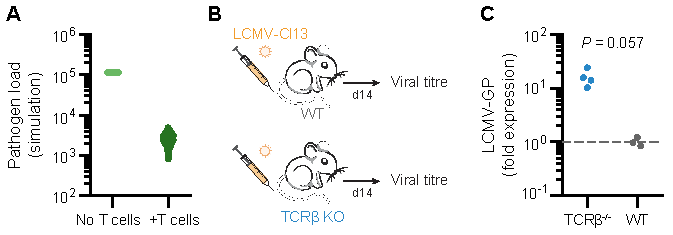
\includegraphics[width=0.64\textwidth]{Figures/VE/figS1_WTvsTCRb.pdf}
    \caption[Lack of host T cells leads to higher pathogen loads both \textit{in silico} and \textit{in vivo}]{\textit{Lack of host T cells leads to higher pathogen loads both \textup{in silico} and \textup{in vivo}}. %
    %
    \secbfcolor{(A)}~Pathogen loads at day 15 post-infection in the model when simulated in the absence or presence of effector T cells. %
    %
    \secbfcolor{(B)}~WT and TCR\textbeta{}\KO{} mice (n=3 and n=4, respectively) were infected with LCMV-Cl13, and spleens were harvested at day 14 for viral titre determination. %
    %
    \secbfcolor{(C)}~LCMV-GP RNA relative fold expression, assessed by qPCR. \textit{P}-value computed using non-parametric rank-sum test.}
    \label{fig:VE_supp_noTcells}
\end{figure}

\begin{figure}[h]
    \centering
    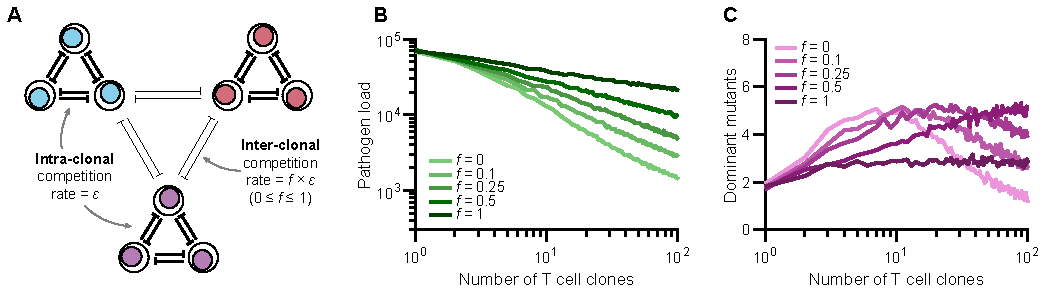
\includegraphics[width=\textwidth]{Figures/VE/figS2_asymComp.pdf}
    \caption[Symmetrical competition within and between T cell clones abolishes peak in mutational burden at intermediate TCR diversity]{\textit{Symmetrical competition within and between T cell clones abolishes peak in mutational burden at intermediate TCR diversity}. %
    %
    \secbfcolor{(A)}~Schematic depicting intra- vs. inter-clonal T cell competition. The inter-clonal competition is assumed to be a fraction, $0\leq f \leq 1$, of the inter-clonal competition rate $\varepsilon$. %
    %
    \secbfcolor{(B)}~Increasing $f$ from 0 (no inter-clonal competition) to 1 (symmetrical competition) reduces the effect of the number of clones $N$ on pathogen control.  %
    %
    \secbfcolor{(C)}~The number of dominant mutants does not peak as a function of TCR diversity when intra- and inter-clonal competition are similar, i.e., as $f\rightarrow1$.}
    \label{fig:VE_supp_asymComp}
\end{figure}

%%

\subsection{Model design}
\label{sec:VE_modelDesign}

The system of ODEs that describes the computational model in Eqs.~\eqref{eq:VE_E}-\eqref{eq:VE_P} were, in part, written as such in order to satisfy two important limits. The first limit considers the case where all effector T cell clones are identical and therefore have the same specificity for a given strain $j$. That is,
%
\begin{equation*}
   k_{1j} = k_{2j} = ... =  k_{Nj} \quad \equiv \quad k_{*j}.
\end{equation*}
%
In this case, the competition between these identical T cell clones would be fully symmetrical (since they would have the same antigen specificity), i.e., $\omega_{in} = 1, \; \forall \; i, n\in\{1,\dots,N\}$. Within this framework, the model should also be equivalent to a model with a single effector T cell clone ($N=1)$, denoted by $\tilde{E}$. To check this, we verified that the dynamics of the sum of identical clones, $E_{\textup{tot}} = \sum_i E_i$, are the same as those produced by $\tilde{E}$ whose specificity for strain $j$ is $1/k_{*j}$. The dynamics of this latter one-clone model are given by
%
\begin{align}
    \dv{\tilde{E}}{t} &= \sigma_E + r_E \tilde{E} \sum_{j=1}^{M(t)}\left(\frac{P_j}{P_\textup{tot} + k_{*j}} \right) -\delta_E \tilde{E} - \varepsilon \tilde{E}^2, \label{eq:VE_Etilde_E} \\[0.5em]
    \dv{P_j}{t} &= r_P \frac{P_j}{P_{\textup{tot}}+P_h} - \delta_P P_j - \kappa_P \tilde{E} \frac{P_j}{P_{\textup{tot}} + k_{*j}}. \label{eq:VE_Etilde_P}
\end{align}
%
By substituting $k_{ij} = k_{*j}$ and $\omega_{in} = 1$ in the original model of Eq.~\eqref{eq:VE_E} and writing it with respect to $\dv*{E_{\textup{tot}}}{t}$, we obtain
%
\begin{align*}
    \dv{E_{\textup{tot}}}{t} &= \sum_{i=1}^N \dv{E_i}{t} \\
    &= \sum_{i=1}^N \left( \frac{\sigma_E}{N} + r_E E_i \sum_{j=1}^{M(t)}\left(\frac{P_j}{P_\textup{tot} + k_{*j}} \right) -\delta_E E_i - \varepsilon E_i \sum_{n=1}^N E_n \right) \\[0.5em]
    &= \sigma_E + r_E E_{\textup{tot}} \sum_{j=1}^{M(t)}\left(\frac{P_j}{P_\textup{tot} + k_{*j}} \right) -\delta_E E_{\textup{tot}} - \varepsilon E_{\textup{tot}}^2,
\end{align*}
%
which, when setting $E_{\textup{tot}} = \tilde{E}$, matches exactly with Eq.~\eqref{eq:VE_Etilde_E}. Similarly, by applying these substitutions to Eq.~\eqref{eq:VE_P}, we obtain
%
\begin{align*}
    \dv{P_j}{t} &=r_P \frac{P_j}{P_{\textup{tot}}+P_h} - \delta_P P_j - \kappa_P \sum_{i=1}^{N}\left(E_i \frac{P_j}{P_{\textup{tot}} + k_{*j}} \right) \\[0.5em]
    &= r_P \frac{P_j}{P_{\textup{tot}}+P_h} - \delta_P P_j - \kappa_P E_{\textup{tot}} \frac{P_j}{P_{\textup{tot}} + k_{*j}}.
\end{align*}
%
This in turn matches exactly with Eq.~\eqref{eq:VE_Etilde_P} when setting $E_{\textup{tot}} = \tilde{E}$. It follows that when all effector T cell clones are identical, the two models are equivalent and the first limiting case is satisfied.

In the second limiting case, we apply a similar logic by making all pathogen strains to be identical, implying that any given T cell clone $i$ will be equally specific for all strains. By ignoring the time dependency of the maximum number of strains $M$ resulting from any new mutation event, we have
%
\begin{equation*}
   k_{i1} = k_{i2} = ... =  k_{iM} \equiv k_{i*}.
\end{equation*}
%
In this case, the model should be equivalent to a model with a single pathogen strain ($M=1)$, denoted by $\tilde{P}$. As before, we verified that the dynamics of the sum across all strains, $P_{\textup{tot}} = \sum_j P_j$, are the same as those produced by $\tilde{P}$, where the specificity of T cell clone $i$ for $\tilde{P}$ is equal to $1/k_{i*}$, by considering the one-strain model given by
%
\begin{align}
    \dv{E_i}{t} &= \frac{\sigma_E}{N} + r_E E_i \frac{\tilde{P}}{\tilde{P} + k_{i*}} -\delta_E E_i - \varepsilon E_i \sum_{n=1}^N \omega_{in} E_n, \label{eq:VE_Ptilde_E} \\[0.5em]
    \dv{\tilde{P}}{t} &= r_P \frac{\tilde{P}}{\tilde{P}+P_h} - \delta_P \tilde{P} - \kappa_P \sum_{i=1}^{N}\left(E_i \frac{\tilde{P}}{\tilde{P} + k_{i*}} \right). \label{eq:VE_Ptilde_P}
\end{align}
%
By substituting $k_{ij} = k_{i*}$ in Eq.~\eqref{eq:VE_E} of the original model and ignoring the time dependency of $M$,  we obtain
%
\begin{align*}
    \dv{E_i}{t} &= \frac{\sigma_E}{N} + r_E E_i \sum_{j=1}^{M}\left(\frac{P_j}{P_\textup{tot} + k_{i*}} \right) -\delta_E E_i - \varepsilon E_i \sum_{n=1}^N \omega_{in} E_n \\[0.5em]
    &= \frac{\sigma_E}{N} + r_E E_i \frac{P_\textup{tot}}{P_\textup{tot} + k_{i*}} -\delta_E E_i - \varepsilon E_i \sum_{n=1}^N \omega_{in} E_n,
\end{align*}
%
which, when setting $P_{\textup{tot}} = \tilde{P}$, matches exactly Eq.~\eqref{eq:VE_Ptilde_E}. Similarly applying these substitutions to Eq.~\eqref{eq:VE_P} and writing it with respect to $\dv*{P_{\textup{tot}}}{t}$, we obtain
%
\begin{align*}
    \dv{P_{\textup{tot}}}{t} &= \sum_{j=1}^{M} \dv{P_j}{t} \\[0.5 em]
    &= \sum_{j=1}^{M} \left( r_P \frac{P_j}{P_{\textup{tot}}+P_h} - \delta_P P_j - \kappa_P \sum_{i=1}^{N}\left(E_i \frac{P_j}{P_{\textup{tot}} + k_{i*}} \right) \right) \\[0.5em]
    &= r_P \frac{P_{\textup{tot}}}{P_{\textup{tot}}+P_h} - \delta_P P_{\textup{tot}} - \kappa_P \sum_{i=1}^{N}\left(E_i \frac{P_{\textup{tot}}}{P_{\textup{tot}} + k_{i*}} \right).
\end{align*}
%
This in turn matches exactly Eq.~\eqref{eq:VE_Ptilde_P} when setting $P_{\textup{tot}} = \tilde{P}$. This means that when all strains are identical, the two models are equivalent and the second limiting case is also satisfied.

Note that the second limiting case would not have been satisfied if $P_{\textup{tot}}$ in the denominator of the terms involved in effector T cell proliferation and T cell-dependent pathogen clearance (i.e., in $P_{\textup{tot}} + k_{ij}$), were replaced with $P_j$. In other words, if the proliferation of, and clearance by, T cells that are induced by a single pathogen strain were completely independent from the presence and abundance of other variants of that pathogen, then the model would depend arbitrarily on the number of strains despite all variants being physiologically indistinguishable. Similarly, if we had replaced $P_{\textup{tot}}$ in the denominator of the replication term of pathogen dynamics with $P_j$, the second limiting case would also no longer be satisfied.

By accounting for these limits when developing the model, we avoided generating results that were an artifact of its design. This form, however, introduces competition between different strains of the pathogen since, for example, the replication of a lowly abundant variant is disfavoured over a prominent one as a result of $P_{\textup{tot}}$ in the denominator of pathogen replication in Eq.~\eqref{eq:VE_P}; this in turn gives rise to an interesting result of the model, which is the pathogen intrinsic range of maximum mutational propensity (Figs.~\ref{fig:VE_effectOfBeta} and~\ref{fig:VE_supp_maxMutProp}). This is because, when the pathogen load of an abundant strain is too high, its competitive advantage makes it less likely for other variants to overtake it and thus for additional dominant mutants to arise. If, on the other hand, pathogen replication of a given strain were completely independent from the presence and abundance of other strains, we would expect the number of dominant mutants to more closely resemble the total number of strains arising from the simulations, i.e., we would no longer see a mismatch between these two metrics as we did in our model (Fig.~\ref{fig:VE_noTcells}). This reasoning provides support for our model prediction that T cell-dependent mechanisms contribute to, but cannot fully explain, immune escape, and that these work together with pathogen intrinsic properties to modulate the abundance and evasiveness of escape mutants.

\renewcommand{\thefigure}{\thechapter.\arabic{figure}}
\renewcommand{\figurename}{Figure}
\setcounter{figure}{0}